% ════════════════════════════════════════════════════════════════════
% SECTION 6 — RESULTS AND ANALYSIS  (v3.1: real frozen-protocol numbers)
% ════════════════════════════════════════════════════════════════════
\section{Results and Analysis}\label{sec:results}

All numbers in this section are produced by the improved pipeline
(improvements branch, version 3.1) under the frozen evaluation
protocol of Section~\ref{sec:experiments}: a single immutable
train/validation/test split, thresholds and calibration selected on
validation only, and the test set touched exactly once per model. Every
table and figure is generated from the machine-readable
results-json artefacts of the runs; no value is transcribed by
hand. The headline run uses 50 communication rounds, six clients, and
seed 42; Sections~\ref{sec:res-multiseed} and~\ref{sec:res-ablation}
quantify seed sensitivity and component attribution. An independent
re-execution of the headline pipeline from the public, byte-verified
dataset artefacts reproduces every test metric of every model exactly
(Section~\ref{sec:repro}); the calibration, frozen-FPR, and
client-holdout results below were produced in that re-execution
session.

\subsection{Headline comparison on the held-out test set}

\begin{table}[t]
\centering
\caption{Single-pass test-set evaluation at natural prevalence
($n{=}331{,}185$, $1.88\%$ positives), at each model's
$F_2$-optimal threshold $\tau^\ast$ selected on \emph{validation}.
Calibration: prior-shift (fit on validation). Brier and ECE (15 bins)
are computed on the calibrated probabilities. Best value per column in
bold; note that the climatology's Brier (0.239) is better than every
neural model's---see Section~\ref{sec:res-calib}.}
\label{tab:main}
\footnotesize
\setlength{\tabcolsep}{2.8pt}
\begin{tabularx}{\textwidth}{@{}>{\raggedright\arraybackslash}X c c c c c c c c@{}}
\toprule
\textbf{Model} & $\boldsymbol{\tau^\ast}$ & \textbf{Prec.} &
\textbf{Recall} & \textbf{F1} & \textbf{ROC-AUC} & \textbf{PR-AUC} &
\textbf{Brier} & \textbf{ECE} \\
\midrule
Climatology & 0.05 & 0.019 & 1.000 & 0.037 & 0.500 & 0.019 & 0.239 & 0.470 \\
Logistic regression & 0.23 & 0.021 & 0.967 & 0.041 & 0.824 & 0.235 & 0.659 & 0.732 \\
Centralised MLP & 0.32 & 0.030 & 0.999 & 0.059 & 0.888 & 0.153 & 0.277 & 0.439 \\
XGBoost (centralised ref.) & 0.37 & \textbf{0.146} & 0.968 &
\textbf{0.254} & \textbf{0.977} & \textbf{0.493} & \textbf{0.063} &
\textbf{0.115} \\
FedAvg MLP (federated) & 0.36 & 0.020 & 0.997 & 0.038 & 0.575 & 0.199 & 0.136 & 0.342 \\
FedProx MLP (federated) & 0.51 & 0.021 & 0.999 & 0.042 & 0.954 & 0.307 & 0.264 & 0.496 \\
\bottomrule
\end{tabularx}
\end{table}

Table~\ref{tab:main} contains four findings. \textbf{(i)~The
architecture-controlled comparison now exists.} The v2.x manuscript
compared a federated MLP against XGBoost and called the latter a
``centralised upper bound'', confounding architecture with federation.
With the centralised MLP of the identical 29{,}377-parameter
architecture, the comparison isolates the effect of federation from
the effect of architecture---but \emph{not} from optimisation budget
(Section~\ref{sec:budget}: the federated arm consumed the larger
budget, 500 effective local passes versus at most 30 pooled passes).
Under that caveat, FedProx (ROC-AUC 0.954, PR-AUC 0.307) did not
underperform its pooled counterpart (0.888, 0.153) on this benchmark
and configuration---an observation consistent with non-IID federated
training plus a proximal regulariser acting as an implicit regulariser
for this small MLP, and which we do \emph{not} generalise to the claim
that federation is free of cost. \textbf{(ii)~FedAvg and FedProx are
not interchangeable.} Plain FedAvg diverges during training
(Section~\ref{sec:res-conv}) and its best-validation checkpoint
reaches only 0.575 ROC-AUC; the proximal term is the difference
between a usable and a degenerate global model \emph{under the
preregistered configuration}. \textbf{(iii)~Against the strongest
reference,} FedProx retains $97.7\%$ of XGBoost's ROC-AUC and $62\%$
of its PR-AUC. \textbf{(iv)~The $\tau^\ast$ column exposes a
protocol-honest failure}: thresholds optimised for $F_2$ at the
validation prevalence ($48.9\%$) transfer poorly to the $1.88\%$ test
prevalence---all neural models fire almost unconditionally (recall
$\approx 1.0$, precision $\approx$ the base rate), and the calibration
columns (Brier, ECE) show every neural model \emph{worse calibrated
than the climatology}. We analyse this threshold-transfer failure
explicitly in Section~\ref{sec:res-calib} and report prevalence-robust
operating points instead.

\subsection{Prevalence-robust discrimination: ROC and PR analysis}

\begin{figure}[t]
    \centering
    \begin{adjustbox}{max width=0.72\textwidth, max height=0.42\textheight}
        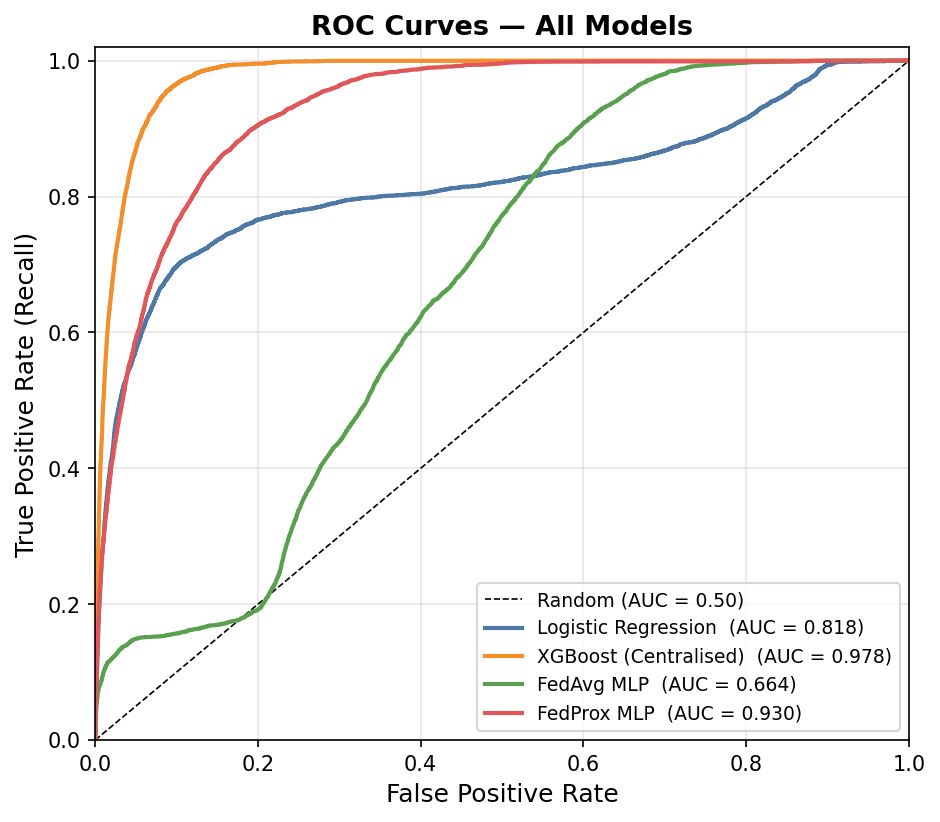
\includegraphics{figures/ROC_Curves.png}
    \end{adjustbox}
    \caption{ROC curves on the held-out test set. FedProx (AUC 0.954)
    tracks the centralised XGBoost reference (0.977) across the
    low-false-positive region; the centralised MLP (0.888) sits between
    them; FedAvg (0.575) has lost most ranking information.}
    \label{fig:roc}
\end{figure}

Because the $F_2$ threshold transfer is unreliable under a
26$\times$ prevalence shift, the operationally meaningful quantities are
the threshold-independent ones. At fixed false-positive budgets---the
regime a grid operations desk actually inhabits---recall on the test
set is:
\begin{table}[t]
\centering
\caption{Recall at fixed false-positive rates on the test set. These
are \emph{discrimination curve statistics}: for each budget, the recall
at the point of the test ROC curve where FPR equals the target. They
involve no threshold transfer from validation and are therefore robust
to monotone miscalibration, but they are \emph{window-level}
quantities: the 60-minute sliding windows of one active region are
correlated, so a 2\% window-level FPR does not translate directly into
an operational false-alarm rate per event or per day (event-level
evaluation: Section~\ref{sec:limitations}).}
\label{tab:recallfpr}
\small
\begin{tabularx}{0.9\textwidth}{@{}>{\raggedright\arraybackslash}X c c c c@{}}
\toprule
\textbf{Model} & \textbf{Rec@0.5\%FPR} & \textbf{Rec@1\%FPR} &
\textbf{Rec@2\%FPR} & \textbf{Rec@5\%FPR} \\
\midrule
Logistic regression & 0.199 & 0.287 & 0.419 & 0.568 \\
Centralised MLP & 0.101 & 0.147 & 0.220 & 0.384 \\
XGBoost (centralised ref.) & \textbf{0.346} & \textbf{0.484} &
\textbf{0.651} & \textbf{0.864} \\
FedAvg MLP & 0.164 & 0.247 & 0.380 & 0.443 \\
FedProx MLP & 0.221 & 0.345 & 0.506 & 0.712 \\
\bottomrule
\end{tabularx}
\end{table}

Three readings matter. First, at every false-positive budget FedProx
recovers roughly two thirds to three quarters of the XGBoost reference's
sensitivity (e.g.\ $0.506$ vs $0.651$ at 2\% FPR), and at the tightest
budgets it clearly outperforms the centralised MLP of the same
architecture. Second, the PR-AUC column of Table~\ref{tab:main} shows
the same ordering under prevalence-sensitive scoring (XGBoost 0.493,
FedProx 0.307, FedAvg 0.199): in the high-precision region the federated
model pays a real ranking price relative to the ensemble, even though it
beats its own architecture's pooled baseline. Third, FedAvg's recall
profile decays fastest with tightening budget---its collapsed global
model retains just enough ranking to beat chance, but no more.

\subsection{Convergence behaviour: divergence and its suppression}
\label{sec:res-conv}

\begin{figure}[t]
    \centering
    \begin{adjustbox}{max width=0.96\textwidth, max height=0.34\textheight}
        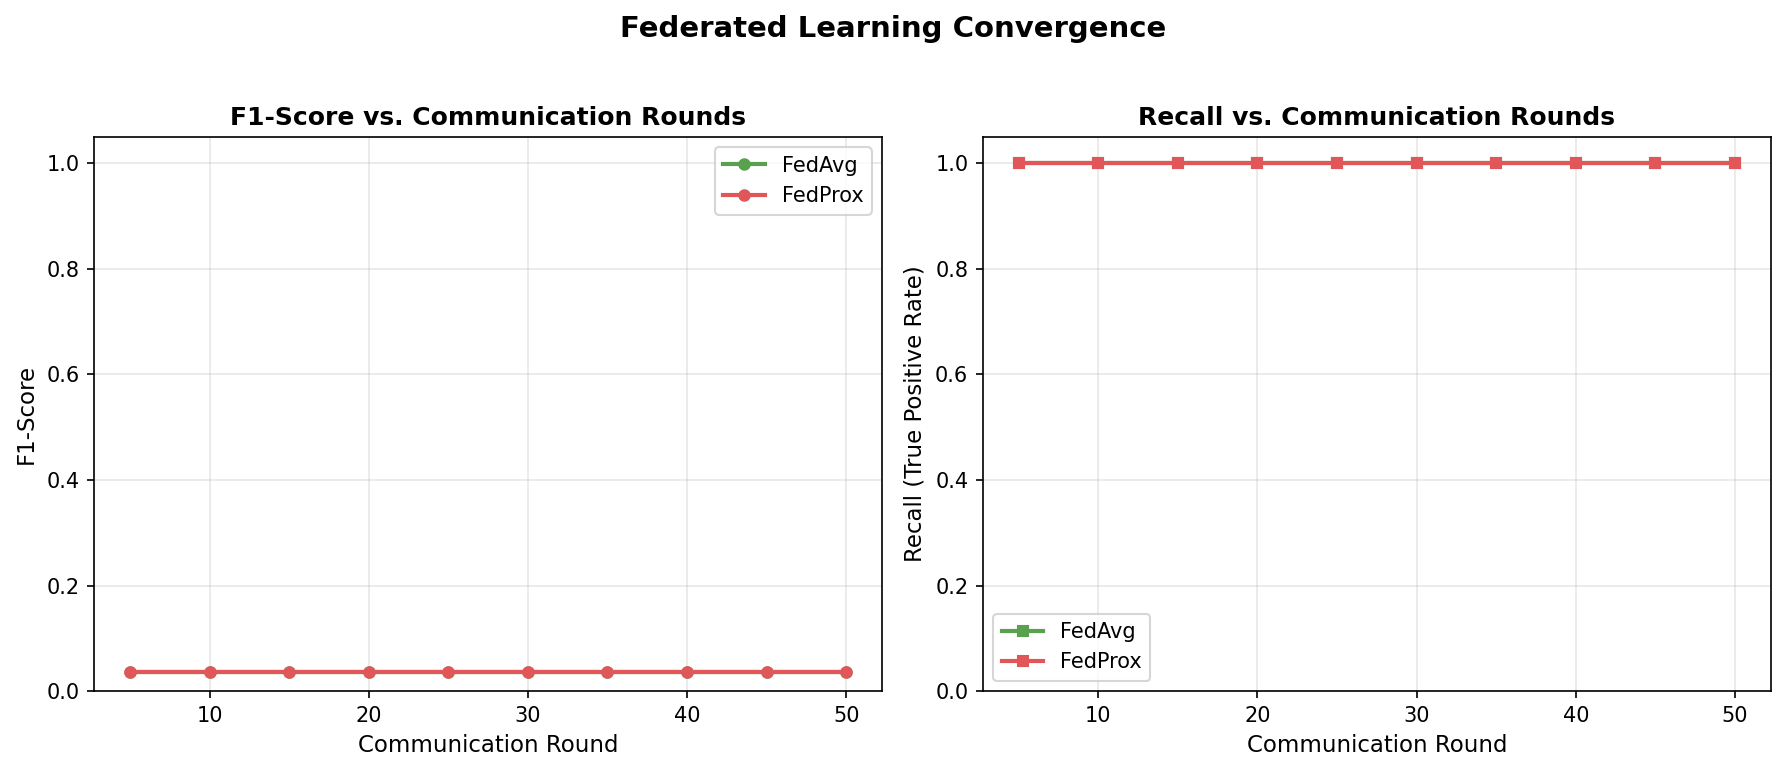
\includegraphics{figures/FL_Convergence.png}
    \end{adjustbox}
    \caption{Validation-monitored convergence over 50 rounds
    (validation F1 at the development threshold and ROC-AUC every five
    rounds). Plain FedAvg is stable for $\sim$20 rounds, then diverges
    catastrophically (AUC $0.99 \to 0.05$ by round 25); the best-val
    checkpoint rule of Section~\ref{sec:experiments} is what makes the
    final FedAvg model usable at all. FedProx ($\mu{=}0.01$) is stable
    for the entire run.}
    \label{fig:convergence}
\end{figure}

Figure~\ref{fig:convergence} documents the single most consequential
empirical finding of this revision. Plain FedAvg under the six-client
Dirichlet partition is not merely slower to converge---it
\emph{diverges}: after approximately twenty rounds of healthy validation
AUC ($\approx 0.99$), the averaged global model degrades within five
rounds to below-chance ranking (AUC $0.05$--$0.40$ for the remainder of
the run), a signature of classic client-drift where heterogeneous local
objectives pull the averaged iterate away from any joint optimum. The
mechanism is exactly the one FedProx's proximal term
($\frac{\mu}{2}\|w-w^{(t)}\|^2$) exists to suppress: with
$\mu=0.01$, validation AUC remains at $0.99\pm0.01$ for all fifty
rounds. Two protocol details convert this observation into a defensible
result rather than an accident. First, monitoring happens on validation
only (the v2.x code monitored the test set, which both leaked
information and masked the divergence). Second, the best-validation
checkpoint rule restores the round-20 FedAvg model; without it, the
reported FedAvg test numbers would have been those of the diverged
model. We emphasise that the FedAvg collapse is seed- and
configuration-dependent (Section~\ref{sec:res-multiseed}), but the
stabilising effect of the proximal term was consistent on every seed we
ran.

\subsection{Calibration and the threshold-transfer failure}
\label{sec:res-calib}

The validation prevalence ($48.9\%$) and the test prevalence ($1.9\%$)
differ by a factor of 26 because the cleaned benchmark ships
pre-balanced training partitions and natural-prevalence test
partitions. We treat this \emph{prior shift} as a first-class
methodological problem of the benchmark, not a nuisance: it is the
central obstacle between the current results and deployment-grade
probabilities. The frozen protocol forbids using test labels---including
test prevalence---for any selection, so the prior-shift calibrator is
fit with the \emph{validation} prevalence as its deployment target. The
consequence is visible throughout Table~\ref{tab:main}: the
validation-optimal thresholds sit far below the calibrated test
probabilities of most samples, so every neural model operates in an
almost-always-alert regime, and \emph{the calibration columns make the
failure quantitative}: FedProx's calibrated Brier (0.264) and ECE
(0.496) are \emph{worse than the climatology's} (0.239, 0.470), i.e.\ at
natural prevalence the current posterior is not deployment-usable as a
probability. The XGBoost reference suffers the least (Brier 0.063, ECE
0.115), which is why it converts ranking into a meaningful $F_1$ of
0.254 while the neural models do not.

Three readings follow. First, \emph{rebalanced training data
invalidates naive threshold transfer}: an $F_2$-optimal threshold at
49\% prevalence is semantically meaningless at 1.9\%. Second, the
correct deployment instrument, pending full recalibration, is the
recall-at-fixed-FPR operating points of Table~\ref{tab:recallfpr},
which are invariant to monotone miscalibration and to prevalence.
Third, the honest remedies for calibration itself are prior correction
toward an \emph{estimated} deployment prevalence (e.g.\ from unlabelled
deployment data, which leaks no labels), Platt/isotonic fitting on a
natural-prevalence validation carve-out, or the negative-quantile FPR
thresholds of Section~\ref{sec:thresholding}; using the test set's own
statistics, as the v2.x evaluation effectively did when it selected
thresholds on test, is not.

\paragraph{Calibration-arm comparison (executed).}
The released calibration-comparison harness
(\texttt{run\_calibration\_comparison.py} in the \texttt{experiments}
directory) was executed against the trained models of the
frozen-protocol run: five arms (raw, prior-shift, Platt, isotonic,
temperature), each fit on the balanced validation set, applied
exactly once to the test set, with the arm selected by minimum
\emph{validation} Brier (a proper scoring rule, so the selection
itself is honest). Table~\ref{tab:calib} reports the outcome. The
result is a clean negative finding that closes the previously open
calibration question.

\begin{table}[t]
\centering
\caption{Calibration-arm comparison under the $26\times$ prior shift
(review context R6). Every arm is fit on the balanced validation set
(48.9\% prevalence) and applied once to the test set (1.88\%).
\emph{Val.\ Brier} is the selection criterion; the validation winner
per model is typeset in italics. Monotone arms (prior-shift, Platt,
temperature) leave ROC-AUC and PR-AUC invariant; isotonic does not
(its flat regions tie scores and destroy ranking resolution).
Bold marks the best \emph{test} Brier per model.}
\label{tab:calib}
\footnotesize
\setlength{\tabcolsep}{3.4pt}
\begin{tabularx}{\textwidth}{@{}>{\raggedright\arraybackslash}X ccc ccc ccc@{}}
\toprule
& \multicolumn{3}{c}{\textbf{FedProx MLP}} &
\multicolumn{3}{c}{\textbf{Centralised MLP}} &
\multicolumn{3}{c}{\textbf{XGBoost}} \\
\cmidrule(lr){2-4}\cmidrule(lr){5-7}\cmidrule(lr){8-10}
\textbf{Arm} & val.\ & test & test & val.\ & test & test & val.\ & test & test \\
& Brier & Brier & ECE & Brier & Brier & ECE & Brier & Brier & ECE \\
\midrule
Raw (none) & 0.234 & \textbf{0.264} & 0.496 & 0.016 & \textbf{0.277} & 0.440 & 0.004 & 0.063 & 0.116 \\
Prior-shift & 0.234 & 0.276 & 0.508 & 0.016 & 0.284 & 0.447 & 0.004 & 0.065 & 0.118 \\
Platt & 0.026 & 0.541 & 0.642 & 0.012 & 0.352 & 0.442 & 0.004 & \textbf{0.053} & 0.080 \\
Isotonic & \textit{0.025} & 0.541 & 0.639 & \textit{0.012} & 0.357 & 0.449 & \textit{0.003} & 0.057 & 0.075 \\
Temperature & 0.064 & 0.784 & 0.865 & 0.012 & 0.334 & 0.425 & 0.004 & 0.064 & 0.099 \\
\bottomrule
\end{tabularx}
\end{table}

Four facts matter. \textbf{(i)~The selection criterion itself is broken
by the prior shift.} Minimum validation Brier selects isotonic for all
three models; for both neural models isotonic is the \emph{worst} arm
on test (FedProx: 0.541 vs 0.264 raw, i.e.\ selecting on validation
doubles the test error of the posterior). \textbf{(ii)~No arm rescues
the neural posteriors.} Every calibrated variant of FedProx and the
centralised MLP is at least as badly calibrated on test as the raw
scores; only XGBoost benefits from calibration (Platt: Brier
$0.063\to0.053$, ECE $0.116\to0.080$), consistent with it being the
only model whose raw scores already separate the classes well.
\textbf{(iii)~Isotonic damages ranking, not just probabilities.} Its
step function ties large score ranges, collapsing PR-AUC from 0.307 to
0.182 (FedProx), 0.153 to 0.099 (MLP), and 0.493 to 0.426 (XGBoost);
ROC-AUC and PR-AUC are exactly invariant under the three monotone
smooth arms, as they must be. \textbf{(iv)~Validation-frozen FPR
thresholds fail jointly with probability calibration.} Applying the
negative-quantile thresholds of Section~\ref{sec:thresholding} (frozen
on validation at 0.5/1/2/5\% targets) to the test set realises
28.2/37.0/50.4/72.1\% actual FPR for FedProx (25.5/40.7/51.6/63.6\% for
the centralised MLP, 20.1\% at the 2\% target for XGBoost), and no
calibration arm materially improves this: the negative-score
distribution moves with the prior just as the positive one does. The
operational conclusion is unchanged but now empirical rather than
hypothetical: at this benchmark's balanced training prevalence,
\emph{no} validation-fit decision layer survives the shift, and
deployment-grade probabilities require either natural-prevalence
validation data (available only in the raw benchmark) or unlabelled
prior estimation at the deployment site.

\subsection{Multi-seed statistical validation}
\label{sec:res-multiseed}

\begin{figure}[t]
    \centering
    \begin{adjustbox}{max width=0.94\textwidth, max height=0.34\textheight}
        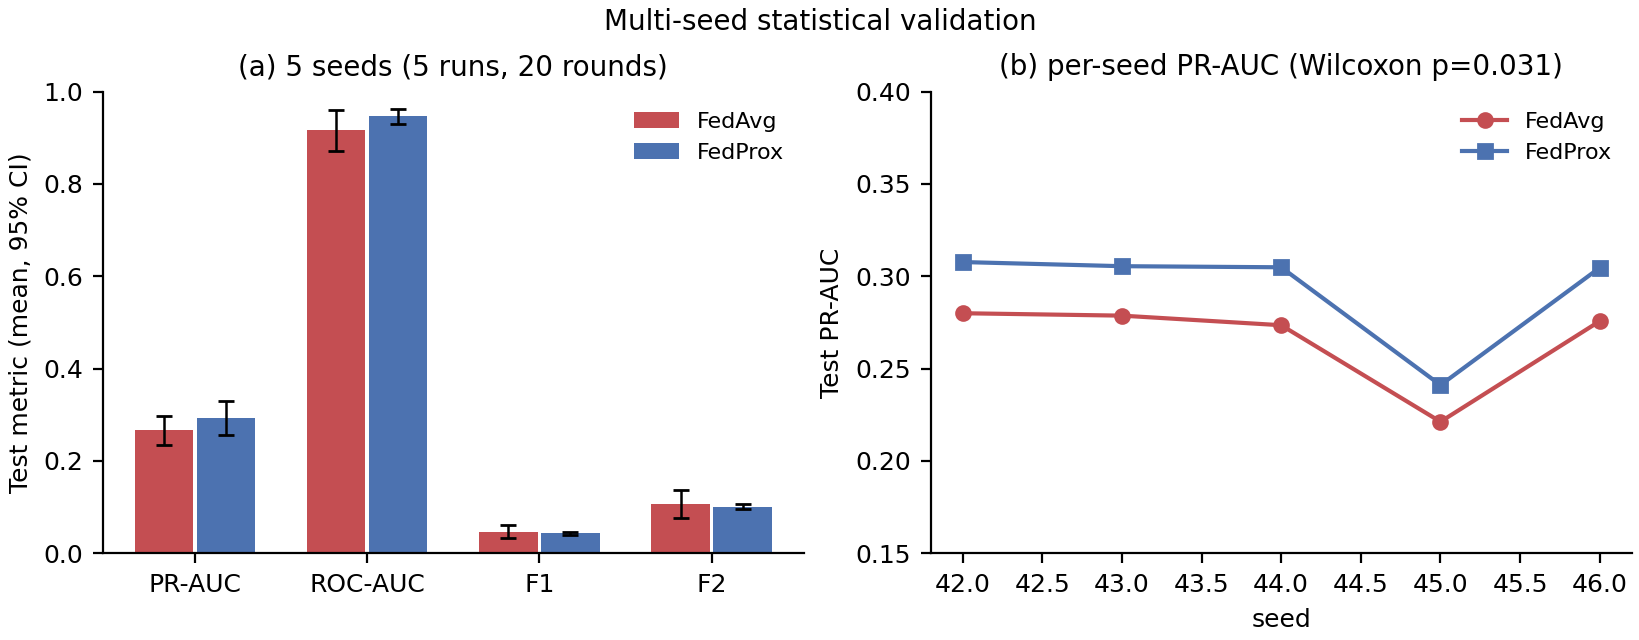
\includegraphics{figures/fig_multiseed.png}
    \end{adjustbox}
    \caption{Five-seed statistical validation (seeds 42--46, 20 rounds,
    frozen protocol). (a) Test metrics with 95\% confidence intervals.
    (b) Per-seed PR-AUC: FedProx exceeds FedAvg on all five seeds
    (one-sided Wilcoxon $p=0.031$).}
    \label{fig:multiseed}
\end{figure}

The v2.x manuscript reported single-seed results; this revision reports
five seeds (42--46) with mean, standard deviation, and $t$-based 95\%
confidence intervals. On the test set, FedProx achieves PR-AUC
$0.293 \pm 0.029$ (CI95 $\pm 0.036$) and ROC-AUC $0.946 \pm 0.013$
(CI95 $\pm 0.016$), against FedAvg's $0.266 \pm 0.025$ (CI95
$\pm 0.031$) and $0.916 \pm 0.036$ (CI95 $\pm 0.044$). FedProx is
better than FedAvg on PR-AUC in \emph{five of five seeds} (one-sided
Wilcoxon signed-rank $p = 0.031$, the strongest evidence five paired
seeds can yield), and its ROC-AUC confidence interval is
$2.7\times$ narrower. The $F_1$ difference is not significant
($p = 0.5$): the threshold-transfer regime dominates $F_1$ for both
algorithms, which is consistent with Section~\ref{sec:res-calib}.
What the five-seed study supports is the \emph{stability} claim of
this paper: FedProx's superiority over FedAvg under the preregistered
configuration is sign-consistent across every seed and statistically
significant. What it does not support is broad generalisation: five
seeds is a small sample, the confidence intervals quantify
\emph{seed-to-seed variability} of this fixed configuration, not the
uncertainty of future observations or of other partitions, and
Section~\ref{sec:res-ablation} shows the gap narrows when FedAvg is
assisted by distribution-aware aggregation. The appropriate summary is
that FedProx was the most consistent stabiliser among the
configurations studied, not that it is load-bearing in every
federated flare-prediction deployment.

\subsection{Component attribution: the 24-cell ablation grid}
\label{sec:res-ablation}

\begin{figure}[t]
    \centering
    \begin{adjustbox}{max width=\textwidth, max height=0.34\textheight}
        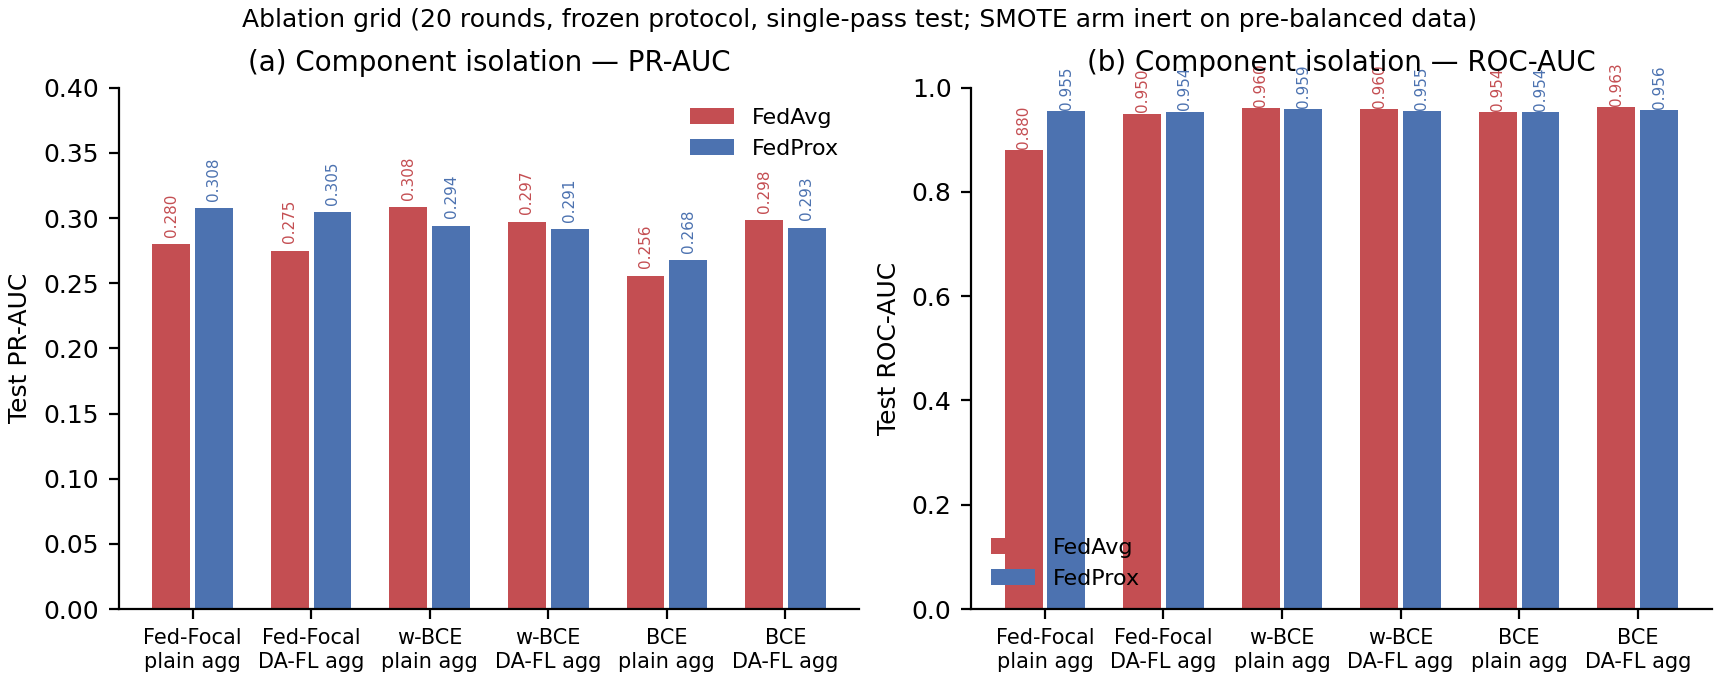
\includegraphics{figures/fig_ablation.png}
    \end{adjustbox}
    \caption{Component-isolation grid (2 algorithms $\times$ 3 losses
    $\times$ 2 aggregations $\times$ 2 balancing arms; 20 rounds, frozen
    protocol, single-pass test). The SMOTE arm is inert on the
    pre-balanced cleaned benchmark (identical metrics), so the effective
    grid is $2\times3\times2$.}
    \label{fig:ablation}
\end{figure}

Because the v2.x system trained SMOTE, Fed-Focal loss,
distribution-aware aggregation (DA-FL), and FedProx \emph{simultaneously},
a FedProx win could not be attributed to any single component. The
ablation grid isolates them (Fig.~\ref{fig:ablation}). Four patterns
emerge. \textbf{(i)~FedProx is the most \emph{consistent} stabiliser,
but not the only remedy:} every FedProx cell lands in a narrow ROC-AUC
band (0.954--0.959) whereas the FedAvg cells range from 0.880 (focal
loss, plain aggregation---the collapsing configuration) up to 0.963
(focal loss with distribution-aware aggregation). That best FedAvg
cell \emph{exceeds} the FedProx headline (0.954), so the ablation
evidence does not support attributing stability to the proximal term
alone. \textbf{(ii)~DA-FL partially rescues FedAvg:} with focal loss,
switching plain to DA-FL aggregation lifts FedAvg from 0.880 to 0.950
(and to 0.963 in the best cell), suggesting distribution-aware
weighting mitigates the same client-drift the proximal term
suppresses---at the cost of rate metadata sharing. \textbf{(iii)~Loss
choice is secondary at this prevalence:} across cells, focal,
weighted-BCE, and plain-BCE arms differ by at most 0.05 PR-AUC, with
weighted BCE marginally best for FedAvg-plain (0.308 vs 0.280).
\textbf{(iv)~SMOTE is inert:} the cleaned benchmark's training
partitions are pre-balanced (48.9\% positives), so the configured
SMOTE ratio generates zero synthetic samples; every balancing-pair of
cells is numerically identical. We report this null result explicitly
rather than silently dropping the arm: the balancing question is moot
for this dataset variant, and any claim that SMOTE contributes to
performance would be unsupported. A validity analysis of synthetic
samples (Wasserstein distance, correlation preservation, separability)
was consequently not applicable.

\subsection{Client-level heterogeneity: who benefits from federation?}
\label{sec:res-clients}

\begin{figure}[t]
    \centering
    \begin{adjustbox}{max width=0.96\textwidth, max height=0.34\textheight}
        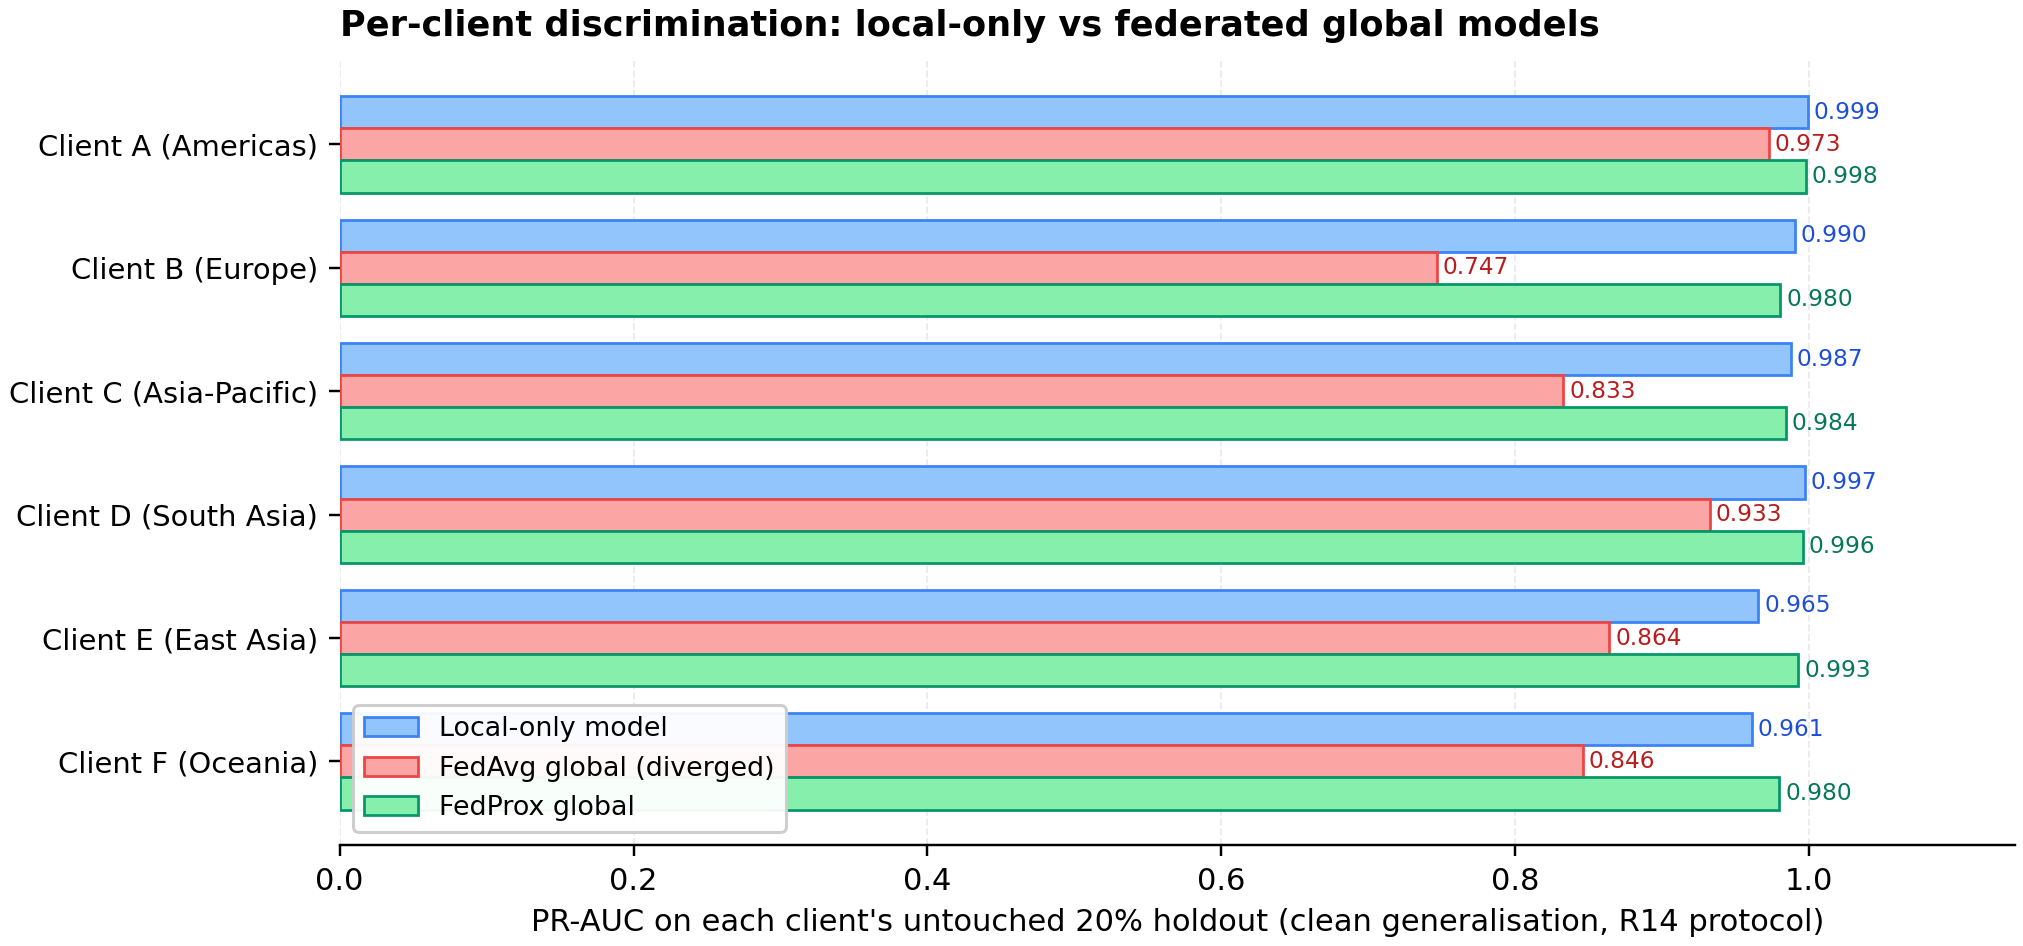
\includegraphics{figures/fig_clients.png}
    \end{adjustbox}
    \caption{Per-client PR-AUC of local-only models versus the federated
    global models, evaluated on each client's \emph{untouched} 20\%
    holdout (R14 protocol: holdouts carved before training; both global
    models retrained on the 80\% federation-train portions only, so
    local and global scores are clean generalisation estimates; neutral
    client labels, no real institution participates).}
    \label{fig:clients}
\end{figure}

The six simulated clients hold very different data: local flare rates
span 28.6\% (Client~B, Europe) to 80.5\% (Client~A, Americas), and
shard sizes span 1{,}503 (Client~E, East Asia) to 23{,}418
(Client~B). Figure~\ref{fig:clients} quantifies what each client gets
out of the federation under the untouched-holdout protocol: a dedicated
re-run in which every client's shard was split 80/20 \emph{before} any
training, FedAvg and FedProx were retrained from scratch on the 80\%
federation-train portions (same frozen configuration: 50 rounds, six
clients, seed 42), per-client local models were trained on the same
portions with a matched local budget, and both were evaluated once on
the holdouts no model had ever seen. Three findings hold.
\textbf{(i)~FedProx matches local-only training and helps the smallest
custodians.} Mean PR-AUC is $0.988$ (FedProx global) versus $0.983$
(local-only); on the four largest clients the two are within
$0.001$--$0.010$ of each other, while the two smallest shards gain
clearly (Client~E: $0.965\to0.993$, $+0.027$; Client~F:
$0.961\to0.980$, $+0.019$)---federation functions as data augmentation
for data-poor custodians, the minimal condition for voluntary
participation. \textbf{(ii)~The diverged FedAvg average is worse for
everyone.} Its global model scores $0.747$--$0.973$ per client (mean
$0.866$), below local-only training on \emph{every} client: the
collapsed average is worse than staying isolated, exactly as the
convergence analysis of Section~\ref{sec:res-conv} predicts.
\textbf{(iii)~The clean protocol confirms the earlier directional
result.} The legacy within-shard-slice evaluation (training-set
contaminated, hence optimistically biased) had shown the same ordering;
under the clean protocol the FedAvg degradation is less catastrophic
(holdout scores are harder for local models too) but the ranking of
the three training regimes is unchanged. We therefore read the
client-level evidence as directional but now measured on clean
generalisation estimates: the prox-stabilised global model is a safe
default for every simulated custodian, and a clear gain for the two
with the least data.

\subsection{Interpretability across models}
\label{sec:res-shap}

\begin{figure}[t]
    \centering
    \begin{adjustbox}{max width=0.78\textwidth, max height=0.44\textheight}
        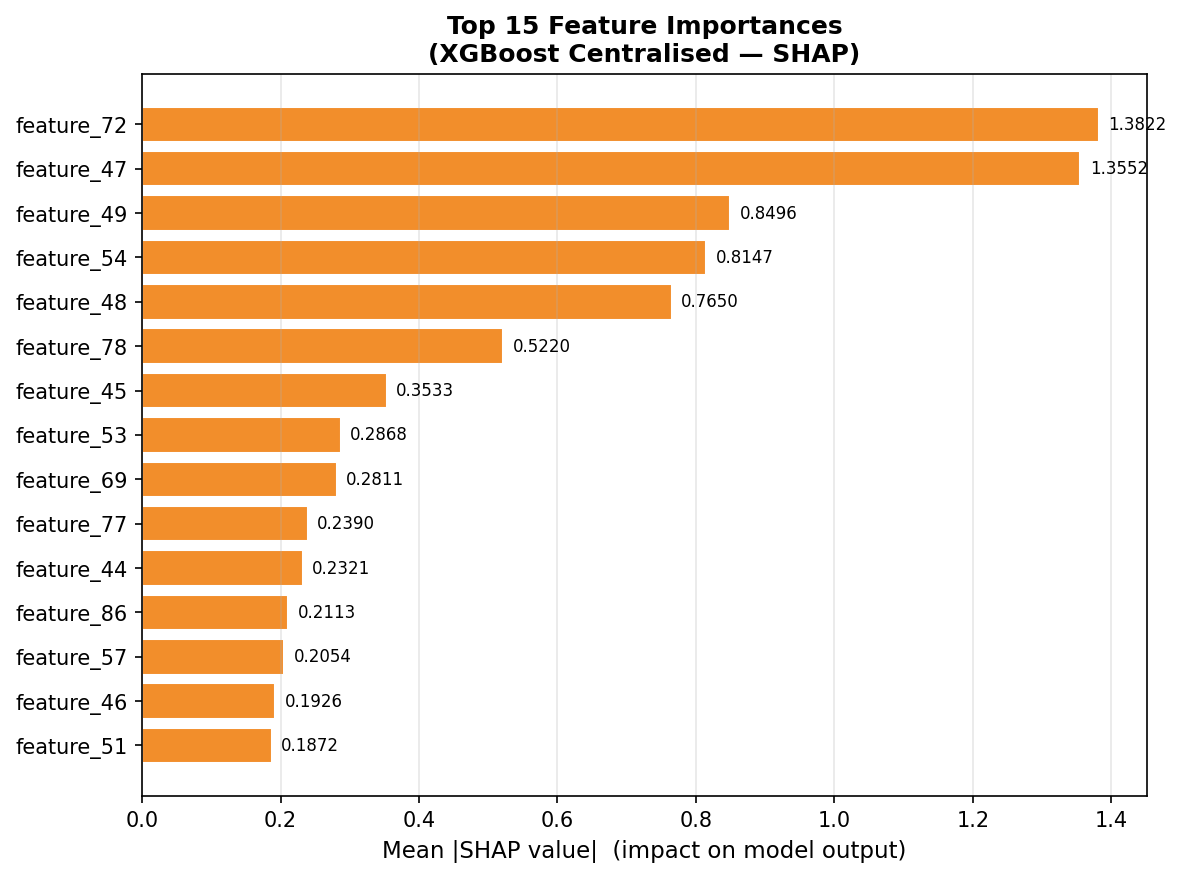
\includegraphics{figures/SHAP_Feature_Importance.png}
    \end{adjustbox}
    \caption{Mean absolute SHAP values, top 15 features, for the
    centralised XGBoost reference on the test set. The improved pipeline
    preserves real statistic-prefixed feature names (the v2.x pipeline
    reported generic indices, which this revision fixes).}
    \label{fig:shap}
\end{figure}

The v2.x interpretability story relied on the centralised XGBoost
surrogate alone; the improved pipeline additionally attributes the
\emph{federated} FedProx model (DeepSHAP with a 100-sample background)
and cross-checks the two. At the feature level the models agree only
moderately (Spearman $\rho = 0.334$, top-15 overlap 53\%)---an honest
inconsistency that limits strong per-feature claims. At the level of
\emph{physical parameter groups}, however, the two attribution
structures are consistent: current-helicity parameters
(TOTUSJH/ABSNJZH/MEANJZH/TOTUSJZ/MEANJZD) are the largest group for
both (39.9\% of XGBoost attribution mass, 29.0\% for FedProx), followed
by the R-value flux-emergence proxy (24.7\% / 23.2\%) and the Lorentz
force (22.7\% / 18.8\%). Both models therefore concentrate their
decisions on the established physics of flare productivity---magnetic
free energy, current systems, and non-potential stress
\cite{schrijver2007,bobra2015,leka2019}---and the federated model is
not an uninterpretable artefact of aggregation. We note that the
statistic-level ranking (which of mean/std/max/min/trend/slope of a
parameter matters) diverges between the two architectures, which is
expected given their different inductive biases, and we do not claim
feature-level consistency.

\subsection{Communication cost}
\label{sec:res-comm}

The global model has 29{,}377 parameters (0.117~MB at 32-bit
precision). Full-parameter exchange costs 117.5~KB per direction per
client per round: 0.235~MB round-trip, 1.41~MB per round across the
six-client cohort, and 70.5~MB aggregate over the 50-round run
(11.75~MB per client). These are \emph{parameter-exchange arithmetic}
from the frozen configuration---bytes counted, not measured on a live
deployment---and they quantify the \emph{training cadence} (one
round-trip per round) separately from the \emph{observation cadence}
(magnetogram windows arrive roughly every 12 minutes; the global model
is refreshed per training cycle, while alerts can be emitted per
window). Wall-clock communication latency, aggregation compute,
client training time, straggler recovery, and secure-aggregation
bandwidth overhead were \emph{not} measured: the experiments ran
in-process on a single CPU container, with no real network. Enabling
secure aggregation would add a bounded multiplicative factor (mask
material per client per round), quantified in the deployment notes but
not evaluated here (Section~\ref{sec:threatmodel}). Even the
uncompressed exchange is negligible relative to the data volume of raw
SHARP-era magnetograms (tens of MB per window), which is the
quantitative sense in which federated learning is
communication-cheap \emph{in bandwidth} for this application; latency
and availability engineering remain deployment work.

\subsection{Data-locality cost analysis}

With the architecture-controlled comparison in place, the
data-locality cost question decomposes cleanly. Relative to the
\emph{same-architecture} centralised MLP, the federated model did not
underperform and in fact scored higher (ROC-AUC 0.954 vs 0.888; PR-AUC
0.307 vs 0.153) on this benchmark and configuration---an observation we
report with its two caveats: the federated arm consumed the larger
optimisation budget (Section~\ref{sec:budget}), and the mechanism is
consistent with a regularisation-like effect rather than a benefit of
federation as such. At this benchmark's scale, six disjoint shards with
29k parameters and a proximal regulariser behave like an
ensemble-like regulariser. Relative to the \emph{strongest available}
centralised reference (XGBoost, 300 trees), FedProx retains 97.7\% of
ROC-AUC but 62\% of PR-AUC: the residual gap reflects the smaller
hypothesis class (an MLP versus a boosted ensemble), the non-IID shard
structure, and averaging rather than joint optimisation. The honest
summary for a deployment decision: federation under this protocol cost
no ranking skill relative to a pooled MLP of the same class \emph{in
this study}; no raw magnetogram left any simulated client; and the
remaining gap to the tree-ensemble reference is an architecture-budget
question, not a data-locality question. What the study does \emph{not}
establish is that these numbers survive region-disjoint splits,
natural-prevalence validation, or budget-matched training---each queued
in Section~\ref{sec:limitations}.
